\documentclass{standalone}
\usepackage{tikz}
\begin{document}

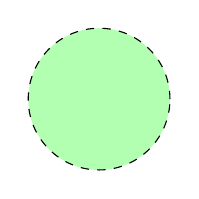
\begin{tikzpicture}
\draw[dashed, fill=green!30] (0, 0) circle (0.9cm);
\end{tikzpicture}

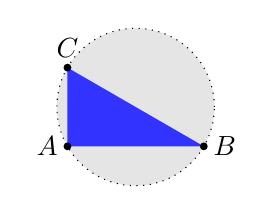
\begin{tikzpicture}
\coordinate[label=left: $A$] (A) at (0, 0);
    \coordinate[label=right: $B$] (B) at ( {sqrt(3)}, 0 );
    \coordinate[label=above: $C$] (C) at (0, 1);

    \draw[fill=gray!20, dotted] ( {sqrt(3)/2}, 0.5 ) circle (1);
    \fill[blue!80] (A) -- (B) -- (C);

    \node at (A)[circle, fill, inner sep=1pt]{};
    \node at (B)[circle, fill, inner sep=1pt]{};
    \node at (C)[circle, fill, inner sep=1pt]{};
\end{tikzpicture}

\end{document}
